\section{Data analysis}
\label{sec:analysis}

In this section we first perform an initial analysis of the data. We check their distributions and assess whether transformations should be performed for better expected results. Furthermore, we can get an initial idea of what variables will perform well by comparing the mean values for people with and without a Nobel Prize. This analysis is done using the R statistical software package.

Next, the logistic regression model is learned on the resulting dataset and evaluated using cross-validation. We experiment with excluding variables that are not relevant and balancing the number of positive and negative examples.

\subsection{Quality assessment}
\label{ssec:quality}

The merged dataset contains two variables that are \emph{fuzzy}: the number of likes on Facebook, which serves as a popularity measure, and the number of results for a specialised Google Scholar search, which serves as a productivity measure. Both might be prone to errors. Furthermore, some normalisation should be performed so that variables with a larger scale do not receive more weight in the final model. Since the university rankings are on a scale of $[0, 100]$ we will transform all variables to that scale.

\subsubsection{Popularity measure}
\label{sssec:popularity}
The popularity measure comes from gathering the number of likes on Facebook. Because this is done automatically and popular names might occur more than ones, we should check for outliers. A boxplot is shown in Figure~\ref{fig:popuInitialBox} and a density plot in Figure~\ref{fig:popuInitialDensity}. We can immediately see a problem: the outlier at 17 million deforms the distribution. It is the result for Einstein, however, and not an error in the data. Manual verification confirmed this for all seemingly high values. In order to solve this without having to remove any data, we perform a transformation using the natural logarithm. Logarithmic transformations are often used to normalise right-skewed distributions. The exact transformation is given by
\begin{equation}
\label{eq:logtransform}
t(x) = \begin{cases} ln(x), & \mbox{if } x \neq 0 \\ 0, & \mbox{if } x = 0 \end{cases}
\end{equation}
in order to correct $ln(0) = -\infty$. The same plots for the resulting distribution are given in Figures~\ref{fig:popuTransformedBox} and \ref{fig:popuTransformedDensity}. While still being far from normal, the outliers are now far less extreme. Next, the results are normalised by dividing by the maximal value and rescaled to $[0, 100]$.
\begin{figure*}[!htb]
    \centering
    \begin{subfigure}[b]{0.3\textwidth}
        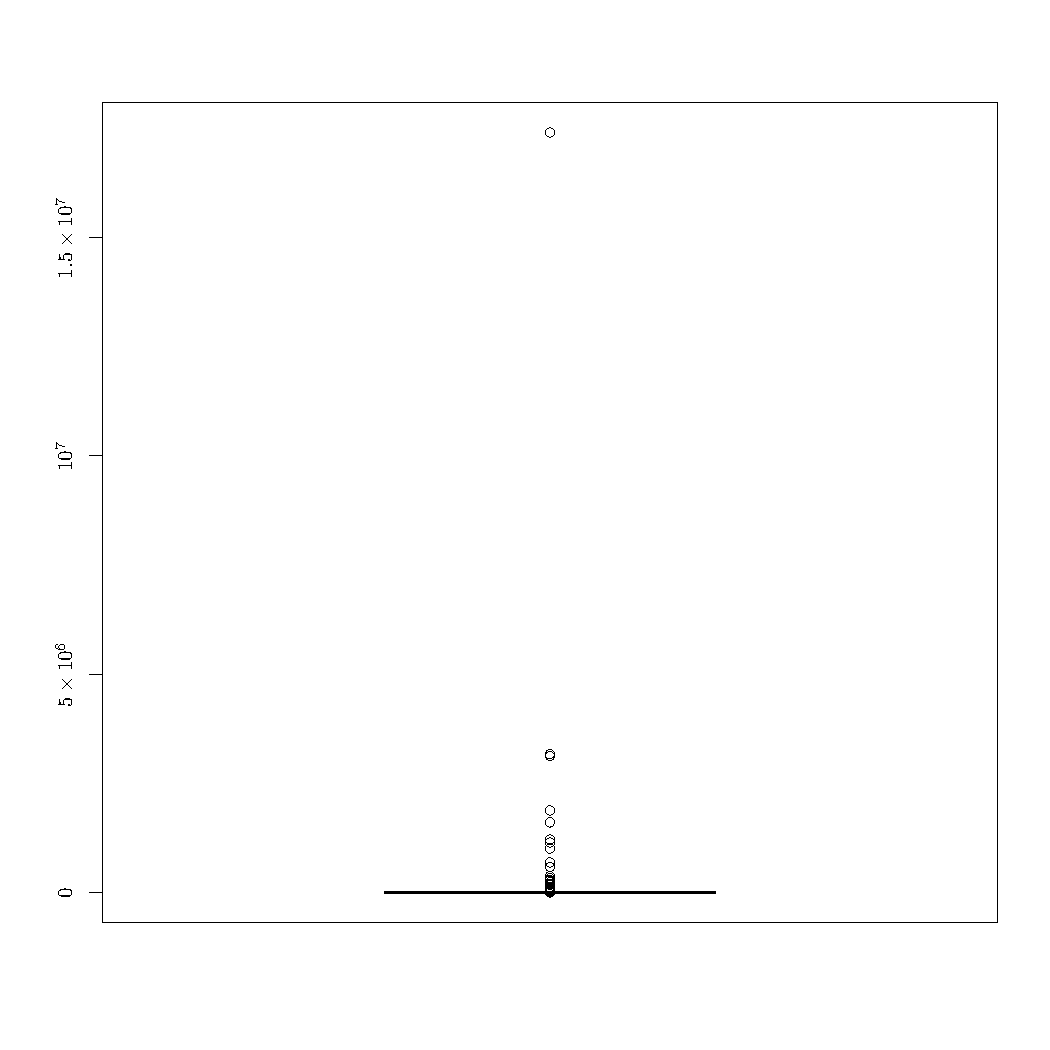
\includegraphics[width=\textwidth]{figures/popuInitialBox}
        \caption{Boxplot}
        \label{fig:popuInitialBox}
    \end{subfigure}
    \quad
    \begin{subfigure}[b]{0.3\textwidth}
        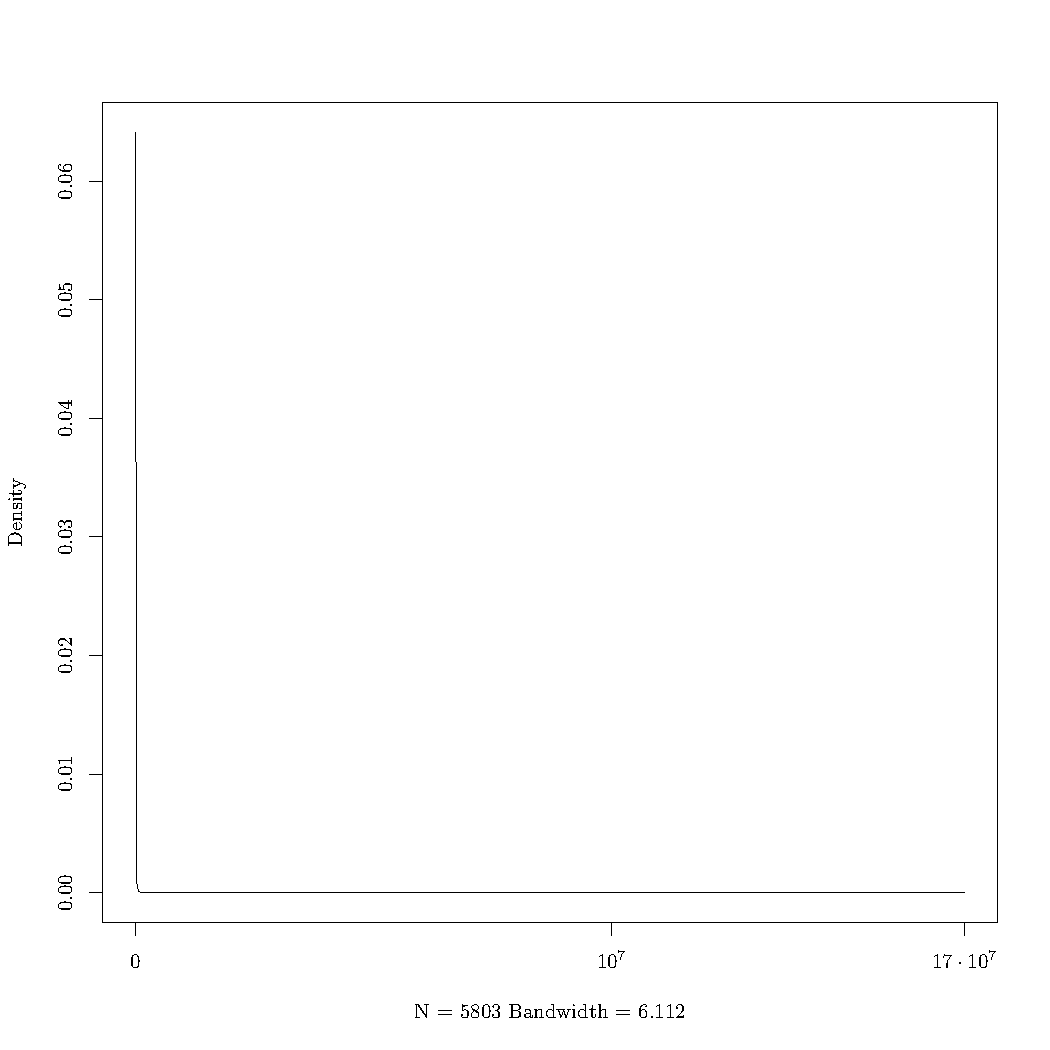
\includegraphics[width=\textwidth]{figures/popuInitialDensity}
        \caption{Density plot}
        \label{fig:popuInitialDensity}
    \end{subfigure}
    \caption{Distribution plots for raw popularity measure.}
\end{figure*}
\begin{figure*}[!htb]
    \centering
    \begin{subfigure}[b]{0.3\textwidth}
        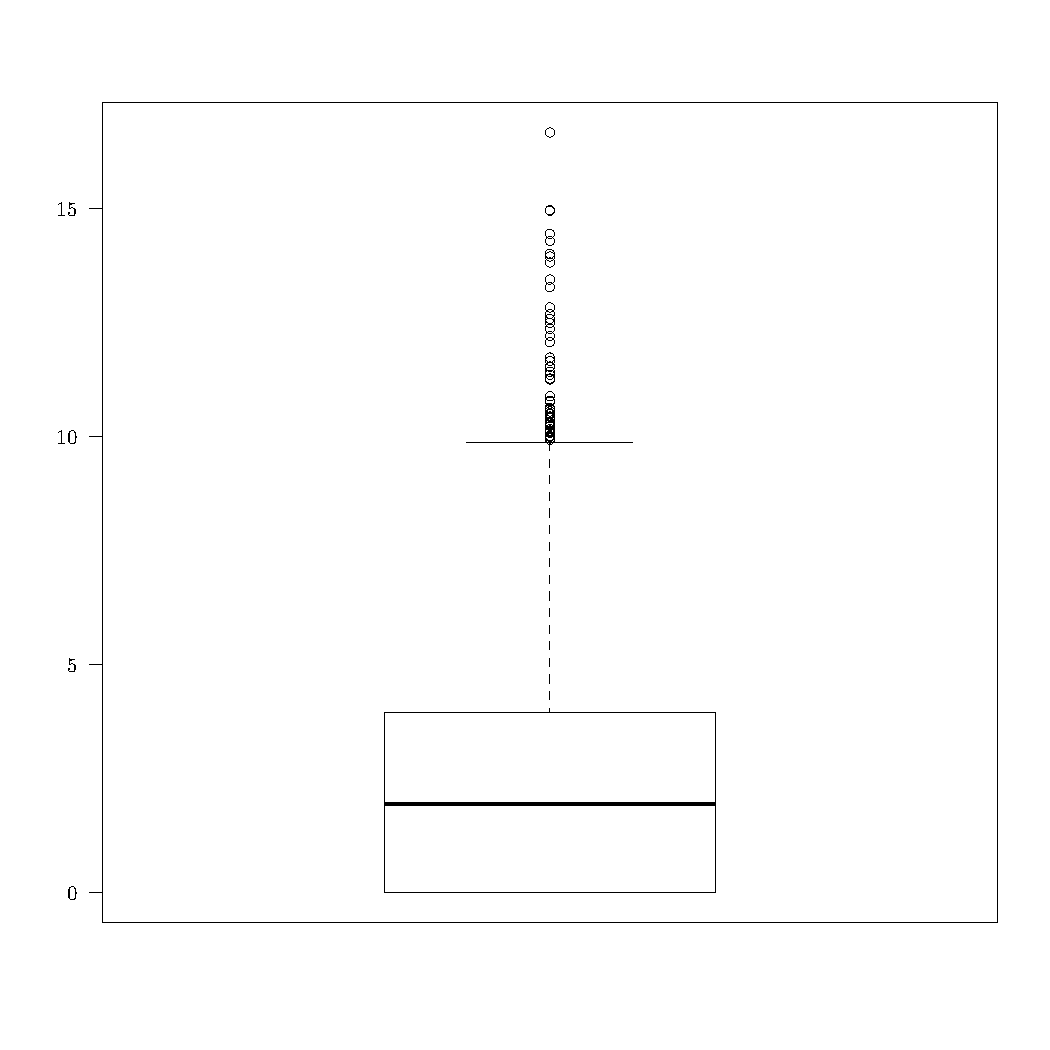
\includegraphics[width=\textwidth]{figures/popuTransformedBox}
        \caption{Boxplot}
        \label{fig:popuTransformedBox}
    \end{subfigure}
	~
    \begin{subfigure}[b]{0.3\textwidth}
        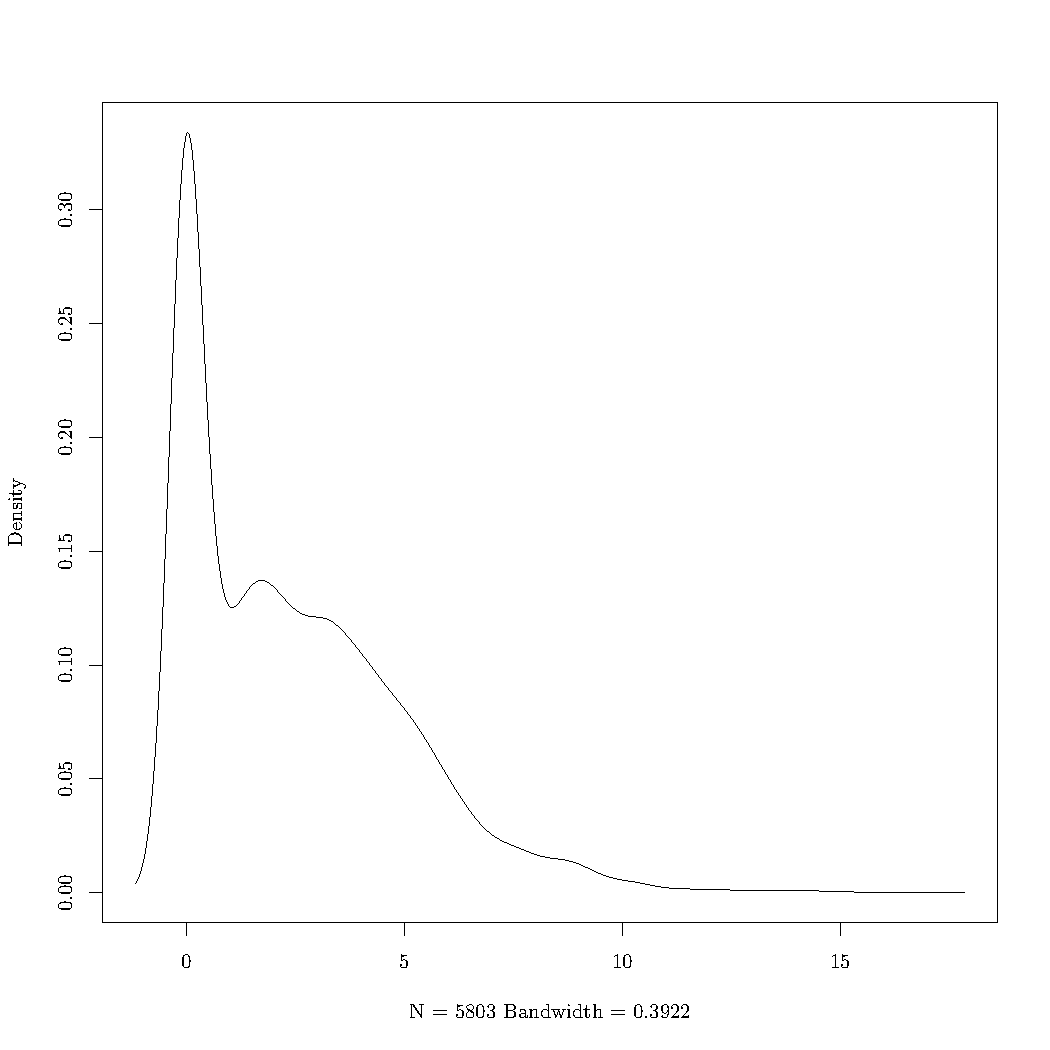
\includegraphics[width=\textwidth]{figures/popuTransformedDensity}
        \caption{Density plot}
        \label{fig:popuTransformedDensity}
    \end{subfigure}
    \caption{Distribution plots for transformed popularity measure.}
\end{figure*}
\begin{figure*}[!ht]
    \centering
    \begin{subfigure}[b]{0.3\textwidth}
        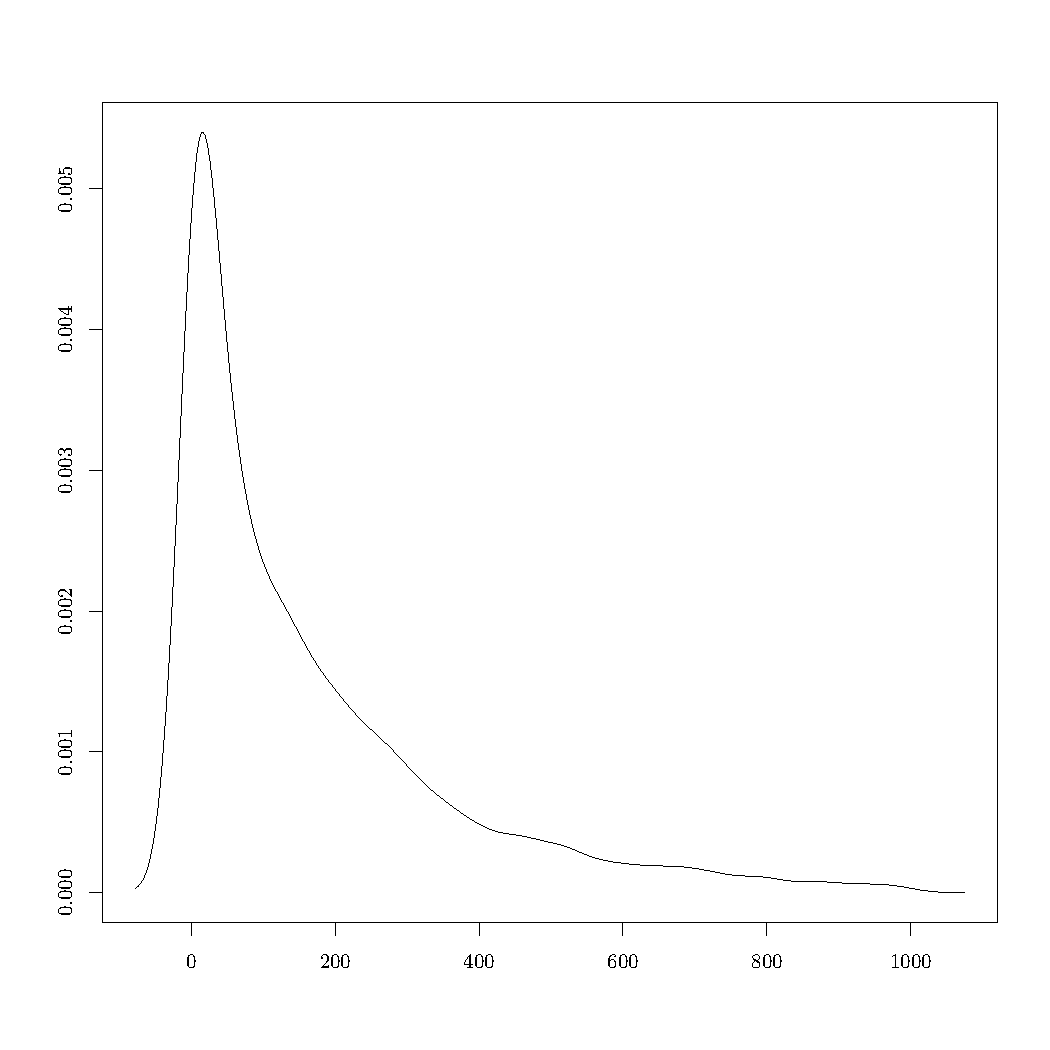
\includegraphics[width=\textwidth]{figures/prodInitialDensity.pdf}
        \caption{Before outlier removal}
        \label{fig:prodInitialDensity}
    \end{subfigure}
    \quad
    \begin{subfigure}[b]{0.3\textwidth}
        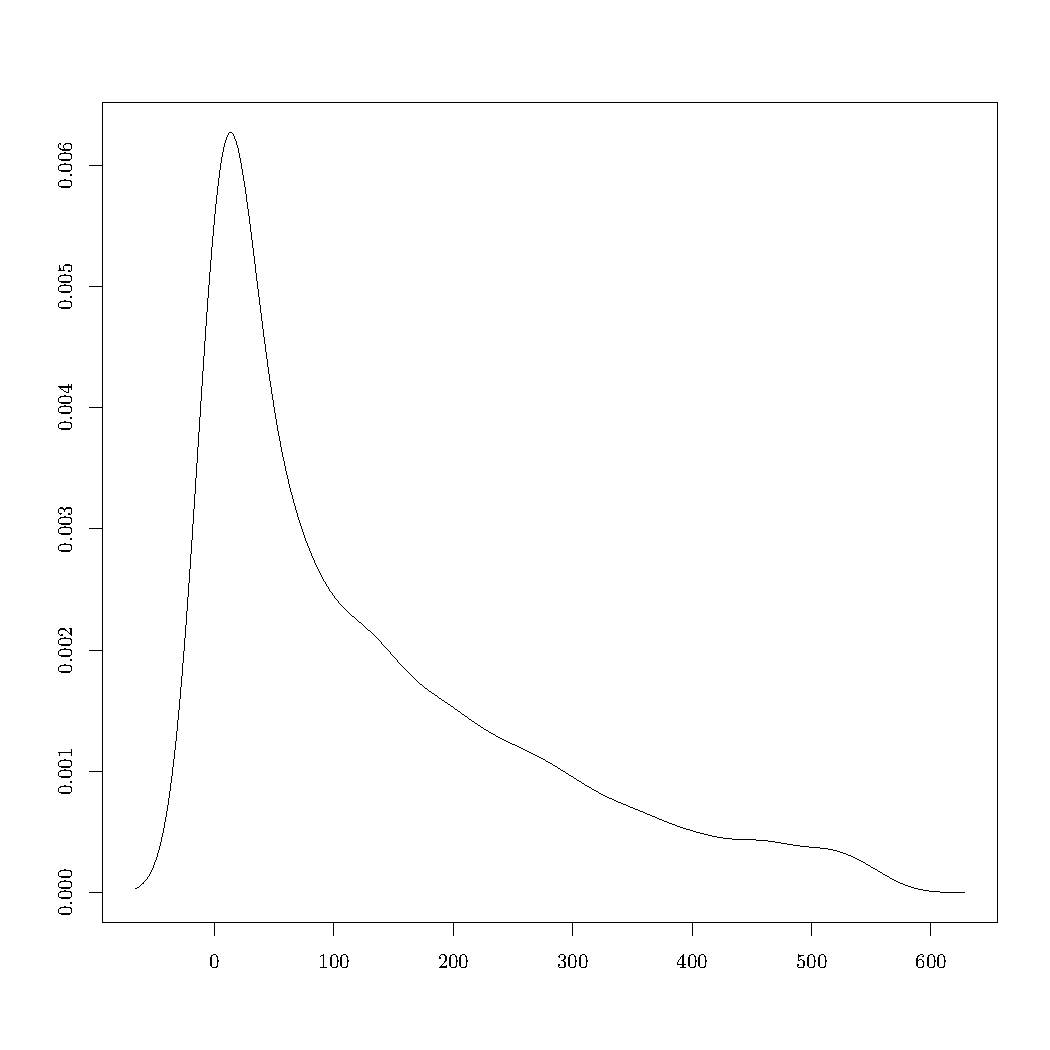
\includegraphics[width=\textwidth]{figures/prodNoOutDensity.pdf}
        \caption{After removing outliers}
        \label{fig:prodNoOutDensity}
    \end{subfigure}
    \caption{Density plots for productivity measure.}
    \label{fig:productivity}
\end{figure*}
In order to get an initial estimate whether it will be significant in the model, we can compare the mean value for winners and non-winners. Since there are sufficient examples, we may assume normality of sampling distributions and perform a standard two-sample $t$ test for unequal variances. The sample means are 
\begin{table}[H]
\centering
\begin{tabular}{c|c}
\textbf{\textsc{Nobel}} & \textbf{\textsc{Non-nobel}} \\ \hline
\rule{0pt}{4mm}23.05663&14.44544\\
\end{tabular}
\end{table} 
\noindent Using R we find that the true means are not equal with confidence level $0.05$, which is what we hoped for the model.

\subsubsection{Productivity measure}
\label{sssec:productivity}
The productivity measure does have outliers, because searching Google Scholar is always a fuzzy search. For example, searching for "Edgar Allen" gives us a result of 996 publications, which is  probably an overestimate. In order to remove these, we perform standard outlier detection, so we remove all points that lie beyond the extremes of the whiskers. The whiskers are extended to 1.5 times the length of the boxes in the boxplot. A density plot of before and after removing the outliers is shown in Figure~\ref{fig:productivity}.
After removing outliers, we rescale the data to $[0, 100]$ per category. The resulting means are given below.
\begin{table}[H]
\centering
\begin{tabular}{c|c}
\textbf{\textsc{Nobel}} & \textbf{\textsc{Non-nobel}} \\ \hline
\rule{0pt}{4mm}25.30257&22.79697 \\
\end{tabular}
\end{table}
\noindent Yet again, we test for equality of means and find that they are not equal, however this time only slightly ($p = 0.03971$, only slightly smaller than the default confidence level $0.05$). Note that before removing outliers they were equal according to the test, which supports our decision to remove outliers.

\subsubsection{Resulting training set}
The resulting training set contains 5486 examples, of which 559 positive and 5243 negative.

\subsection{Learning a model}
Using the generated training dataset, we can begin learning a logistic regression model. In order to better compare the models we learn using different settings, we first need to specify what properties we're looking for. The problem at hand is a hard one, so creating a model with high precision and recall will probably be impossible. Because of the nature of the problem, we want models with a high precision, whereas recall is less relevant. For example, we do not want lots of politicians to be classified as positive, but when one is classified as such we want that prediction to be as accurate as possible.

In order to validate models, we will use 10-fold cross-validation. This is repeated such that the whole dataset was used as an input to the model, trained by other instances. From this estimation, we can estimate precision and recall for the model.

The initial model uses all features and results in the following weights
\begin{table}[H]
\centering
\begin{tabular}{c|c}
\textsc{\textbf{Feature}} ($\mathbf{x}$) & \textsc{\textbf{Weight}} ($\boldsymbol{\beta}$)\\ \hline
\rule{0pt}{4mm}\emph{Intercept}&-2.650\\
Year&-0.520\\
University score&-0.285\\
Popularity&0.789\\
Productivity&0.068\\
\end{tabular}
\end{table}
\noindent which can be interpreted as 
\begin{equation*}
	p(\mathbf{x} = winner) = \frac{1}{1 + e^{-\boldsymbol{\beta}\mathbf{x}}}.
\end{equation*}
We immediately notice that Productivity doesn't have much effect on the result, which we suspected would happen from the low $p$ value for the $t$-test. Performance for this initial model is given in Table~\ref{tbl:initialPerformance}. The relevant percentages are shown in bold. We notice that the recall is low, as expected. This roughly means that if an instance is positive, the model only has 4.59\% chance of discovering this. On the other hand, if an instance is predicted positive, there is a 75\% chance that this is correct, which is not bad at all. 

\begin{table}
\centering
\begin{tabular}{c|l|c|c|c}
\multicolumn{2}{c|}{} & \multicolumn{2}{c|}{\textsc{Actual}}&\\ \cline{3-4}
\multicolumn{2}{c|}{\rule{0pt}{4mm}} &No&Yes&Precision\\ \hline
\multirow{2}{*}{\textsc{Predicted}}&\rule{0pt}{4mm}No&4954&499&90.85\%\\ \cline{2-5}
\rule{0pt}{4mm}&Yes&8&24&\textbf{75.00\%}\\ \hline
&\rule{0pt}{4mm}Recall&99.84\%&\textbf{4.59\%}&\\
\end{tabular}
\caption{Performance for initial model.}
\label{tbl:initialPerformance}
\end{table}

In order to improve on this result, another model was constructed by balancing the number of positive and negative examples: all positive examples were included in the training set and an equal number of negative examples was sampled. This method resulted in a model with higher recall (about 60\%), but far lower precision (also about 60\%). Because the low precision is not what we want, this model was discarded. Next, we attempted to exclude some variables from the training set to create a better model. This resulted in the final model in which Productivity is not included, for which performance can be found in Table~\ref{tbl:resultingPerformance}. The weights of the final model are
\begin{table}[H]
\centering
\begin{tabular}{c|c}
\textsc{\textbf{Feature}} ($\mathbf{x}$) & \textsc{\textbf{Weight}} ($\boldsymbol{\beta}$)\\ \hline
\rule{0pt}{4mm}\emph{Intercept}&-2.651\\
Year&-0.973\\
University score&-0.299\\
Popularity&0.899\\
\end{tabular}
\end{table}


\begin{table}
\centering
\begin{tabular}{c|l|c|c|c}
\multicolumn{2}{c|}{} & \multicolumn{2}{c|}{\textsc{Actual}}&\\ \cline{3-4}
\multicolumn{2}{c|}{\rule{0pt}{4mm}} &No&Yes&Precision\\ \hline
\multirow{2}{*}{\textsc{Predicted}}&\rule{0pt}{4mm}No&4956&499&90.85\%\\ \cline{2-5}
\rule{0pt}{4mm}&Yes&6&24&\textbf{80.00\%}\\ \hline
&\rule{0pt}{4mm}Recall&99.84\%&\textbf{4.59\%}&\\
\end{tabular}
\caption{Performance for final model.}
\label{tbl:resultingPerformance}
\end{table}
